\documentclass[UTF8,a4paper]{ctexart}
\usepackage[margin=1in]{geometry}
\usepackage{threeparttable}
% \usepackage{hyperref}
\usepackage[colorlinks,linkcolor=black,citecolor=black]{hyperref}
\usepackage[section]{placeins}
\usepackage{titlesec}
\usepackage[numbers]{gbt7714}
\usepackage{algorithm}
\usepackage{algpseudocode}
\usepackage{algorithmicx}
\usepackage{amsmath}
\usepackage{float}
\usepackage{array}
\usepackage{graphicx}
\usepackage{subfigure}
\usepackage{fancyhdr}
\usepackage{amssymb}
\usepackage{listings}
\usepackage{color}
\usepackage{bm}
\usepackage{threeparttable}
\usepackage{booktabs}


\floatname{algorithm}{算法}

\definecolor{dkgreen}{rgb}{0,0.6,0}
\definecolor{gray}{rgb}{0.5,0.5,0.5}
\definecolor{mauve}{rgb}{0.58,0,0.82}

\lstset{ %
  language=java,                % the language of the code
  basicstyle=\footnotesize,           % the size of the fonts that are used for the code
  numbers=left,                   % where to put the line-numbers
  numberstyle=\tiny\color{gray},  % the style that is used for the line-numbers
  stepnumber=1,                   % the step between two line-numbers. If it's 1, each line 
                                  % will be numbered
  numbersep=5pt,                  % how far the line-numbers are from the code
  backgroundcolor=\color{white},      % choose the background color. You must add \usepackage{color}
  showspaces=false,               % show spaces adding particular underscores
  showstringspaces=false,         % underline spaces within strings
  showtabs=false,                 % show tabs within strings adding particular underscores
  frame=single,                   % adds a frame around the code
  rulecolor=\color{gray},        % if not set, the frame-color may be changed on line-breaks within not-black text (e.g. commens (green here))
  tabsize=2,                      % sets default tabsize to 2 spaces
  captionpos=b,                   % sets the caption-position to bottom
  breaklines=true,                % sets automatic line breaking
  breakatwhitespace=false,        % sets if automatic breaks should only happen at whitespace
  title=\lstname,                   % show the filename of files included with \lstinputlisting;
                                  % also try caption instead of title
  keywordstyle=\color{blue},          % keyword style
  commentstyle=\color{dkgreen},       % comment style
}

\newcolumntype{L}[1]{>{\raggedright\let\newline\\\arraybackslash\hspace{0pt}}m{#1}}
\newcolumntype{C}[1]{>{\centering\let\newline\\\arraybackslash\hspace{0pt}}m{#1}}
\newcolumntype{R}[1]{>{\raggedleft\let\newline\\\arraybackslash\hspace{0pt}}m{#1}}

\begin{document}


\begin{figure}[ht]
    \centering
    
\includegraphics{titlepage.png}
\end{figure}
\thispagestyle{empty}
\newpage


\tableofcontents
\thispagestyle{empty}
\newpage

\begin{figure}[ht]
    \centering
    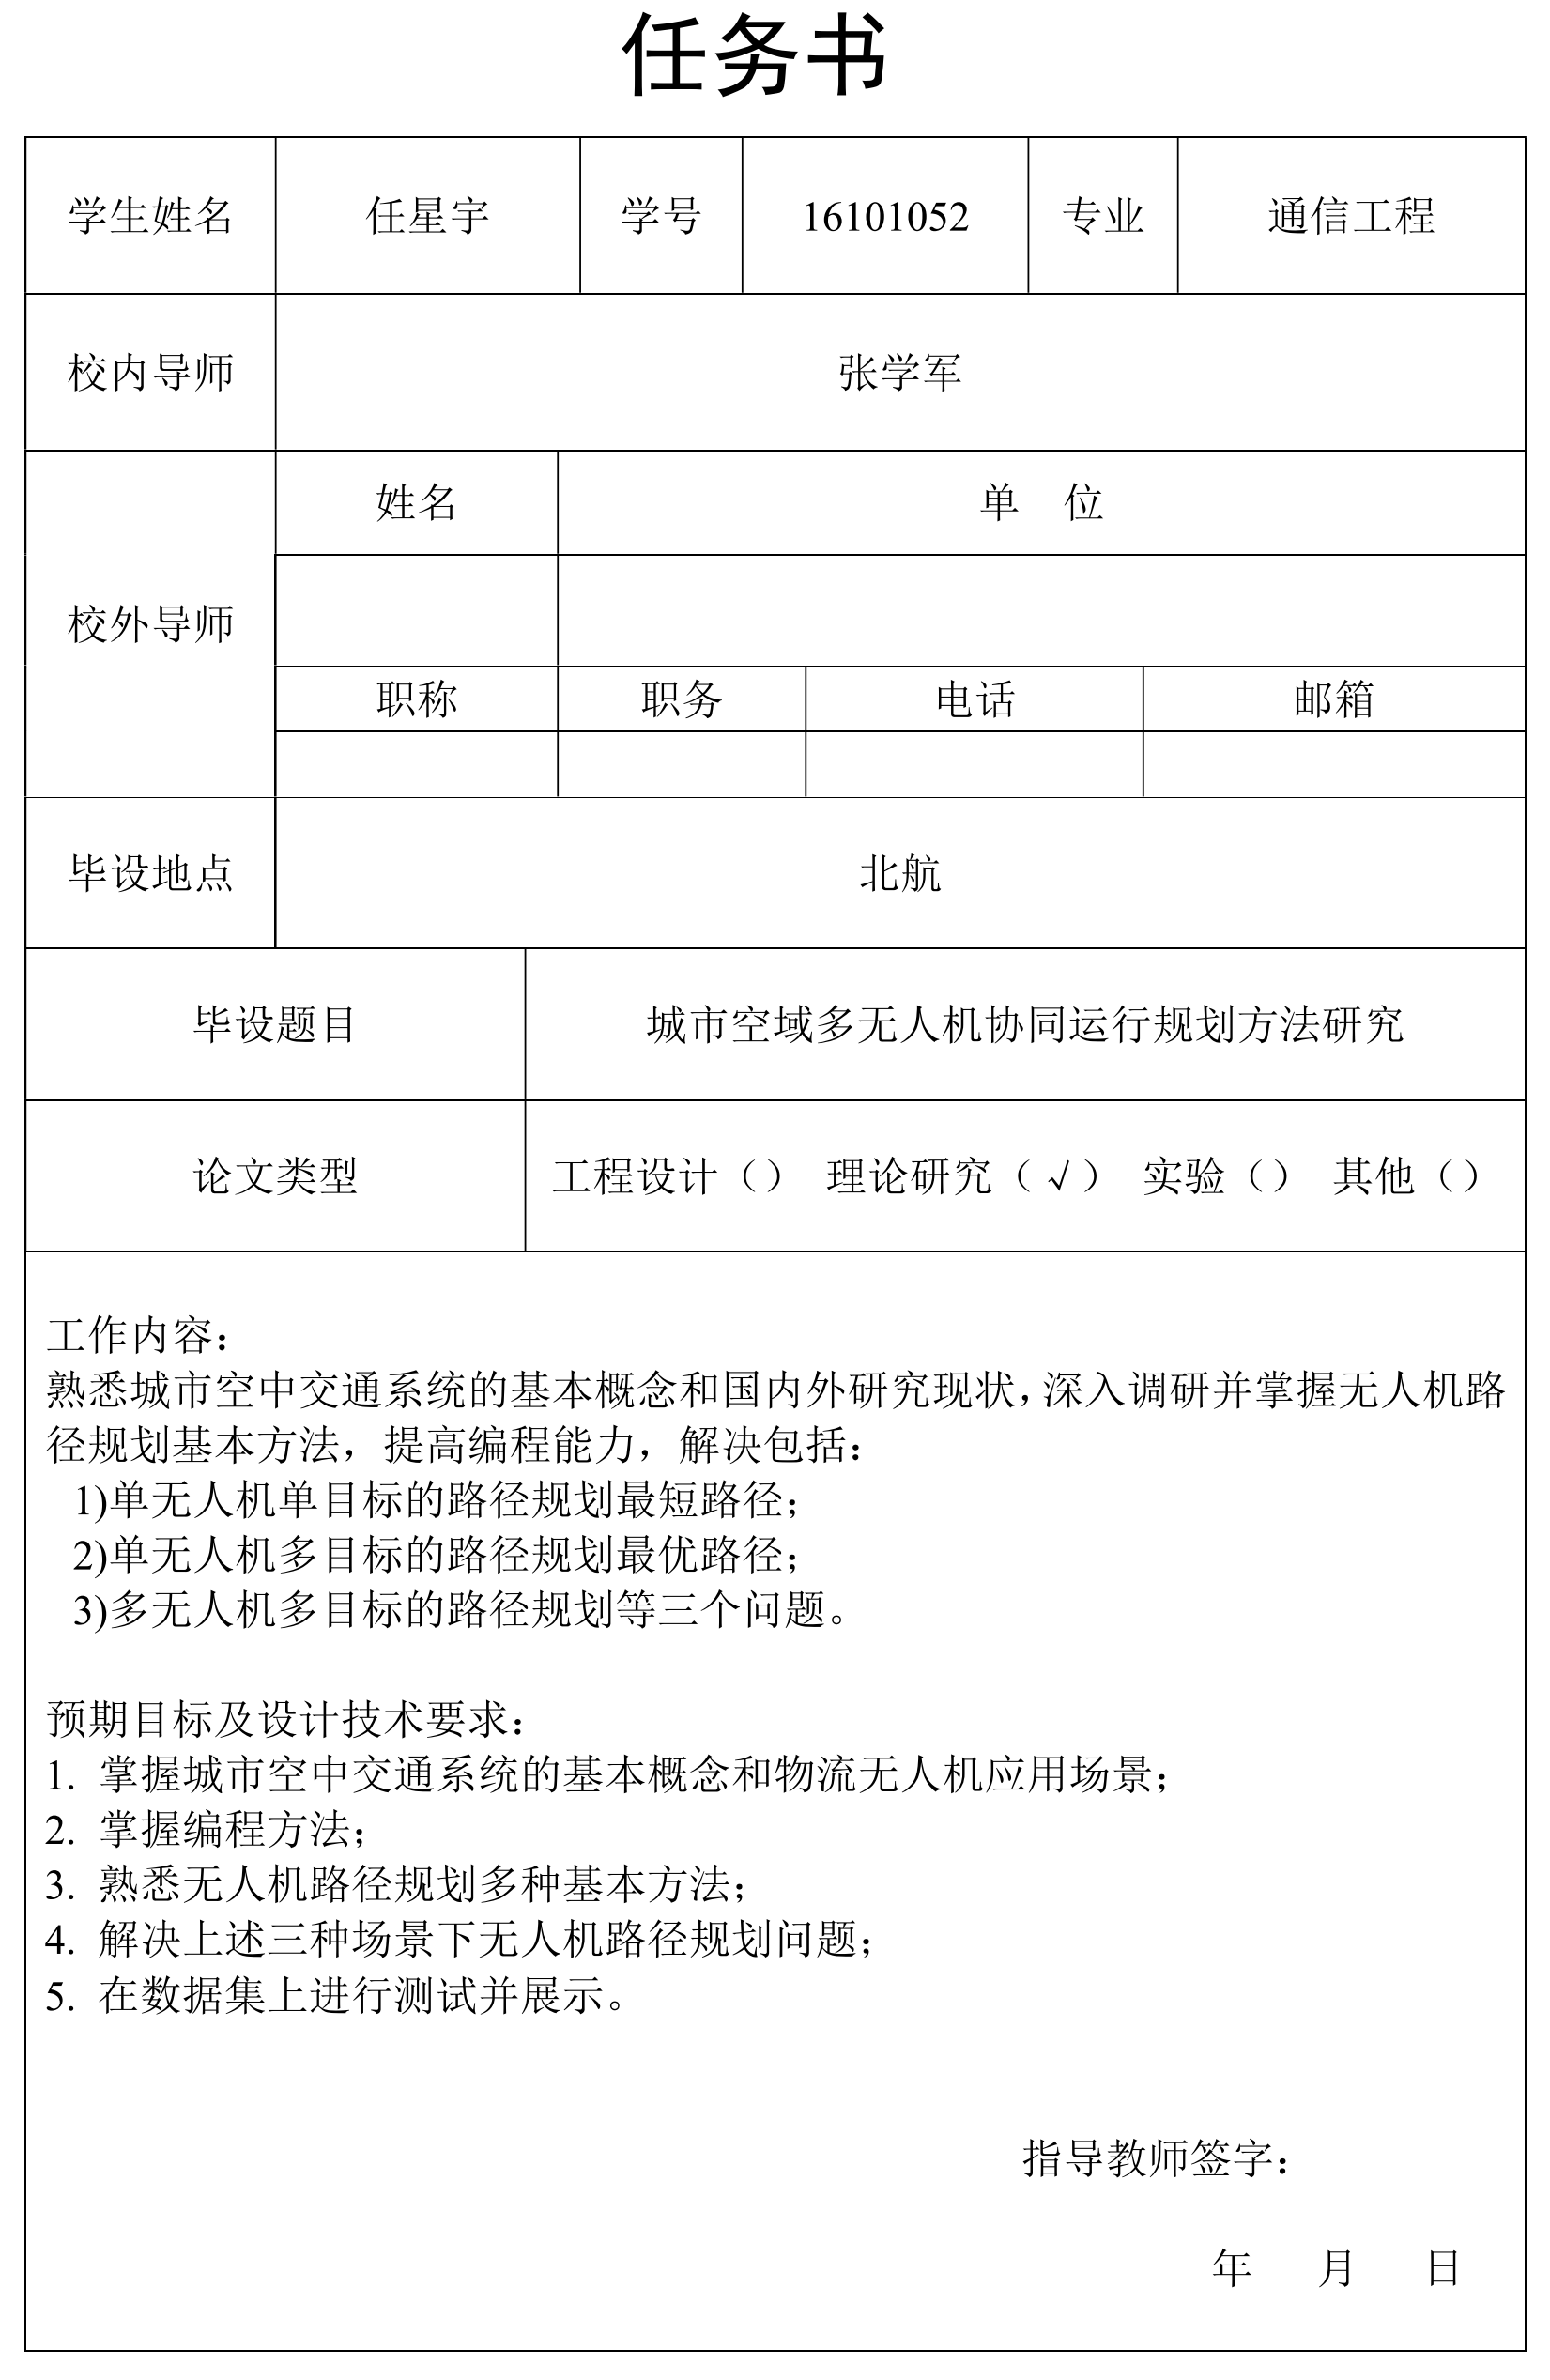
\includegraphics[scale=0.75]{renwushu.png}
\end{figure}
\thispagestyle{empty}
\newpage

\pagestyle{fancy}		%使用fancy页面风格
\rhead{}
\chead{北京航空航天大学电子信息工程学院}			%设置页眉中间
\lhead{}
% \lfoot{\rightmark}			%设置页脚左侧为rightmark
\cfoot{\thepage}			%设置页脚中间为页码
\newpage
\section{毕设工作简介}
\setcounter{page}{1}
\subsection{课题来源、研究目的及意义}
\paragraph{}近年来低空无人机发展迅速,根据中国民航局2019年第一季度无人机云数据统计:运行高度在120m以下的无人机占96.5\%,1000m以下的无人机占据99.9\%.无人机从某特定地点起飞,按照任务要求在复杂空域内运行并到达指定目的地,运行过程中不能给地面人类、空中交通参与者带来威胁,同时规避空域内障碍物风险、潜在威胁区域以及可能的飞行冲突问题,最终满足无人机飞行代价最低~\cite{kopardekar2016unmanned}。
\paragraph{}要解决上述问题,首先,要开展无人机运行安全风险评估研究,从地面、空中两个角度衡量无人机运行所带来的安全隐患,在满足安全性前提下获取无人机自身目标安全水平,评估运行空域的安全状态并生成空域危险等级;其次,基于无人机自身目标安全水平以及空域安全态势要求,开展单架无人机自主飞行路径规划研究,针对二维、三维不同运行场景参数限制,有效规避地形障碍物、空域潜在威胁等因素,为无人机规划最优运行路径;第三,在解决单架无人机最优化运行的基础上,研究多无人机协同路径规划问题并考虑时间因素,在实现无人机自身影响因素建模的前提下,重点解决多无人机时空协同运行问题、飞行冲突及间隔保持问题,为每架无人机规划时空最优运行路径。针对单架无人机路径规划场景数据量大、作用因素多且关联性强、全局范围内寻优复杂等诸多难点问题,首先,根据无人机运行任务需求设计一种离散化的路径特征提取机制,将此类问题转化为多目标大尺度下的联合全局优化,然后构造地形函数并完成所有影响因素的建模;其次,将无人机飞行距离、飞行时间等均作为约束条件,设计目标优化函数并在搜索空间内为其分配搜索阈值;第三,基于指定地形特征及影响因素作用开展最优化运行研究,提出两类适用于二维/三维不同场景下的高效路径规划算法,实现最优解位置的快速定位并得到最优运行路径点序列,实验结果证明算法具有较好的有效性、精确性与鲁棒性。针对多无人机运行规划中自身限制因素建模难、四维协同运行规划难等突出问题~\cite{liuyang}。
\paragraph{}例如亚马逊等公司开发的无人机物流配送即为其中一种应用场景,本课题的背景也是基于物流配送的低空无人机,意图初步实现一种物流管理和路径规划方案。低空环境更接近于路面的路径,但是低空无人机可以经过的空间是三维的,相对地面的车辆,路径限制更少。
\subsection{国内外研究现状}
\paragraph{}关于路径规划,有经典的算法和近年来发展的算法。 经典的算法是基于图论的组合优化问题。涉及的经典算法包括 Dijkstra 算法,Floyd-Warshall 算法,流问题的 Ford-Fulkerson 方法~\cite{introtoalgo}。近年来在经典算法方向的研究也包括利用组合优化的方法,利用整数规划,动态规划等方法,进行路径的规划~\cite{introtoor}。这种方法的原理是在规划空间内用一系列的路径段表征一条运行路径,通过搜索算法寻找最优的路径段实现无人机最佳运行路径的获取,该方向已经成为研究的热点。通过使用 Voronoi 图实现了飞行器的运行规划,此方法是把危险区域、无人机均等同于一个质点并建立 Voronoi 图,然后通过 K 算法寻找最优路径,由于该算法并未涉及无人机自身的参数性能因素,并不符合实际的运行 要求,因此无法真正应用到实际场景中;又进一步的将该算法扩展到了无人直升机的运行规划领域,而且收到了较好的效果,PRM 算法的核心是通过在运动的空间内实施采样,通过采样结果生成路线图,然后基于该路线图进行路径的进一步搜索后得到最佳路径,主要分为学习阶段、查询阶段两个过程;还有一种方法叫可视图法(Visibility Graph, VG)~\cite{2005coordination},将障碍物、危险区域的顶点作为可视图基本元素,由互相可见的顶点生成路线 图,该方法原理简单,执行起来并不复杂,但是当区域内的危险区域、障碍物较多时, 算法的效率急剧下降,需要耗费大量的计算时间;Canny 早在 1987 年就提出了一种 叫做轮廓图的路线图理论,通过映射将高维度规划空间转化为低维度,在低维空间内 找出障碍物对应的边界,即轮廓,然后反复迭代最终得到一维轮廓曲线,进而获取最终的运行路径,该方法的缺陷是当问题维数较高时需要进行多次映射,导致运算量大、耗时长,此方法并不是十分实用;还有一种概率地图法~\cite{zhangyi2007j},在无人机自主运行规划中得 到了广泛的应用,通过该方法使得规划问题的复杂度与规划空间的复杂度不受规划空间维数的影响,因此即使规划空间维度很高时也不会影响算法的执行效率,运算时间几乎不受影响 基于组合优化的经典算法研究在于精确(或较精确)的求解问题,可以保证最优(或对于 NP 难问题求近似最优)~\cite{chenyan2009}。
\paragraph{}而另一种思路和方向是通过类似统计和估计的近似算法,包括蚁群算法,PSO 算法,以及启发式的算法,例如A*算法。这些算法的特点是结果未必正确,精确性和模型个体相关性较大,与计算参数和计算机效果相关性很大,甚至从其算法目的上来说,其追求的就是“近似最优”。 近些年的另一种研究思路是通过人工智能的方法研究路径规划。

\subsection{研究内容简介}
\subsubsection{问题的简述}
\paragraph{}对于地面路径规划的研究已有不少,所以对于无人机的路径规划,其实有其一般性,但是由于无人机这一特殊的对象以及其所运行的环境的不同,这一问题又有其特殊性。
\paragraph{}无人机所运行的环境与地面的路径很多不同,包括\begin{itemize}
    \item 在一些空间内,障碍物并不多,所以我们完全可以用两点之间线段最短来解决这个问题;如果在此环境中使用较为密集的数据单元结构进行计算,那么计算量很大,而且肯定不会比直线段有更近的距离
    \item 在一些环境中,无人机并不是完全自由的,除了建筑物等障碍物之外,由于各种禁飞区和人员密集区的安全考虑,可自由飞行的区域要大打折扣。
\end{itemize}
\subsubsection{图的描述}
\paragraph{}有常见的几种图的表示方法,如下。
\begin{itemize}
    \item 栅格图\label{grid}
          \paragraph{}
          栅格图是一些由特定大小的立方体塞满整个空间的一种图的表示方法,一个立方体有6或8或更多的可运行方向,表示无人机可以从一个方格运行到另一个方格的方向。这种图的好处在于格子之间的路径是确定的,比如对于坐标轴方向的移动,耗费的距离为$a/2$,其中$a$是立方体的边长。但这种图的结构带来的很严重的问题就是数据密度过大,对于一个各个边有100个立方体组成的边来说,它的节点的数量级就已经超过了$10^6$,这种数量是难以进行计算的。但是,如果我们想要以更低的数据密度来进行计算,带来的问题是严重的,比如在一个过大的栅格中有很多房屋,对于无人机配送来说就有很大的误差~\cite{gridsgraph}。
    \item 无向图
          \paragraph{}给定一个图$G=(V,E)$,其中$V$表示的是图的顶点,对应于无人机在运行中需要经过的节点,$E$表示节点之间的边,这是一种最简单的图模型。这种图相对于栅格图,具有更高的抽象,更适合作为数学的研究对象。就其定义而言,顶点的名字在当前并不重要,我们需要的是一个之地啊这些顶点的方法,使用$0,...,V-1$来表述咯咯地那个点。这样描述是为了方便使用数组的索引进行节点的访问,我们知道,在计算机中,数组中下标为$i$的节点的访问速度是$O(1)$,关于这种表示相对于实际生活的差距问题,我们在后续的API中进行处理。无向图其实已经不错,对于大多数问题来说已经够了,图中的节点并不是栅格图中的相邻方格,而是表示某一个地理上的节点,比如一处房屋,或者一个物流配送点。这相对于栅格图有更小的数据密度而不至于失去精确性~\cite{introtoalgo}。
          \paragraph{}
          但是对于生活中的一些问题,无向图又有了缺点。比如车辆上坡和下坡的时间消耗和油耗是不同的,即使是同一条路。这就引出了有向图
    \item 有向图
          \paragraph{}有向图中地每一条边都是有方向的,不仅可以很好地描述各个抽象节点之间地距离,而且可以描述更多地问题,比如单行道,比如同一段上下坡路的不同代价。
          \paragraph{}关于有向图,也有很多研究的形式,我们在这里采用如下规定:
          \begin{itemize}
              \item 没有负边
              \item 不考虑自环
          \end{itemize}
\end{itemize}


\subsubsection{单无人机的单目标路径规划}
\paragraph{}这个问题的主要内容是考虑一个简单的配送站,在规定只有一个目标的情况下,如何从源节点(配送站)将货物送达目标的最优方案问题。
\paragraph{}最优的方案在本研究中是指最短路径。
\paragraph{}关于最短路径的算法,有很多精确的经典算法,比如Dijkstra算法~\cite{felner2011position}和Bellman-Ford算法~\cite{bellman1958routing}。
\paragraph{Dijkstra算法}Dijkstra算法能够解决边权重非负的加权有向图的单起点最短路径问题。其运行的时间复杂度是$O(E\log{V})$.
\paragraph{Bellman-Ford算法}本算法能够解决包含负权重边的加权有向图的单起点最短路径问题。时间复杂度是$O(EV)$.
\paragraph{}对于我们的问题的模型是没有负权重边的,加上时间的考虑,最终使用了Dijkstra算法。其实现见~\ref{sec:dijkstra}.

\paragraph{A*算法}一种启发式的单节点最短路径的算法,关于种种解决方案并没有具体的时间复杂度,但是这种方案有很大的弊端,其一是基于栅格图~\ref{grid}的缺陷,数据密度过大,有很多冗余,使得算法运行非常慢;其二是算法是启发性的,往往并不能得到最短的路径,只是相对短的路径~\cite{astarredbloggames}。


\subsubsection{单无人机的多目标路径规划}
\paragraph{准备}在考虑正式的问题之前,我们先实现一些工具方法。
\subparagraph{Floyd-Warshall算法}Floyd-Warshall 算法采用动态规划方案来解决在一个有向图 $G = (V, E)$ 上每对顶点间的最短路径问题,即全源最短路径问题(All-Pairs Shortest Paths Problem),其中图 $G$ 允许存在权值为负的边,但不存在权值为负的回路。Floyd-Warshall 算法的运行时间为 $Θ(V^3)$。
\subparagraph{}Floyd-Warshall 算法由 Robert Floyd 于 1962 年提出,但其实质上与 Bernad Roy 于 1959 年和 Stephen Warshall 于 1962 年提出的算法相同。其实现见~\ref{sec:floydsolution}.


\paragraph{TSP问题}在存在多个目标的情况下,可以抽象为TSP问题~\cite{tsptheory},又称旅行商问题。给定一系列节点和每对节点之间的距离,求解访问每一座节点一次并回到起始节点的最短回路。它是组合优化中的一个NP困难问题,在运筹学和理论计算机科学中非常重要。已知TSP算法最坏情况下的时间复杂度随着节点数量的增多而成超多项式(可能是指数)级别增长。
\subparagraph{}问题在1930年首次被形式化,并且是在最优化中研究最深入的问题之一。许多优化方法都用它作为一个基准。尽管问题在计算上很困难,但已经有了大量的启发式和精确方法,因此可以完全求解节点数量上万的实例,并且甚至能在误差1\%范围内估计上百万个节点的问题。
\subparagraph{}甚至纯粹形式的TSP都有若干应用,如企划、物流、芯片制造。稍作修改,就是DNA测序等许多领域的一个子问题。在这些应用中,“节点”的概念用来表示客户、焊接点或DNA片段,而“距离”的概念表示旅行时间或成本或DNA片段之间的相似性度量。TSP还用在天文学中,观察很多源的天文学家希望减少在源之间转动望远镜的时间。许多应用(如资源或时间窗口有限)中,可能会加入额外的约束~\cite{worldtsp}。
\subparagraph{}TSP问题可以通过整数规划的方法解决~\cite{papadimi},目前还没有进行整数规划的学习,暂将方程列下:
\begin{align*}
    \min & \sum _{i=1}^{n}\sum _{j\neq i,j=1}^{n}c_{ij}x_{ij}\colon &  &                      \\
         & x_{ij}\in \{0,1\}                                        &  & i,j=1,\ldots ,n;     \\
         & u_{i}\in  \mathbb{Z}                                     &  & i=2,\ldots ,n;       \\
         & \sum _{i=1,i\neq j}^{n}x_{ij}=1                          &  & j=1,\ldots ,n;       \\
         & \sum _{j=1,j\neq i}^{n}x_{ij}=1                          &  & i=1,\ldots ,n;       \\
         & u_{i}-u_{j}+nx_{ij}\leq n-1                              &  & 2\leq i\neq j\leq n; \\
         & 0\leq u_{i}\leq n-1                                      &  & 2\leq i\leq n.
\end{align*}
\subparagraph{}关于TSP问题的是实现见~\ref{sec:solutionTSP}.
\subparagraph{应用场景}除了本文所述的物流规划问题,TSP问题在其他方面也有很多应用。比如飞机航线安排、送邮件、快递服务、设计校车行进路线等等。实际上其应用范围扩展到了许多其他领域。
\subparagraph{}印制电路板转孔是TSP应用的经典例子,在一块电路板上打成百上千个孔,转头在这些孔之间移动,相当于对所有的孔进行一次巡游。把这个问题转化为TSP,孔相当于节点.孔到孔之问的移动时间就是距离。
\subparagraph{}此外,旅行商问题还有电缆和光缆布线、晶体结构分析、数据串聚类等多种用途。更重要的是.它提供了一个研究组合优化问题的理想平台。很多组合优化问题,比如背包问题、分配问题、车间调度问题都和TSP同属NP完全问题,它们都是同等难度的.如果其中一个能用多项式确定性算法解决,那么其他所有的NP完全问题也能用多项式算法解决。很多方法本来是从TSP发展起来的.后来推广到其他NP完全问题上去~\cite{tsp2006}。

\subsubsection{多无人机的多目标路径规划}
\paragraph{}多无人机的路径规划涉及的主要问题是车辆路径规划问题(Vehicle Routing Problem),是TSP问题的一般化,相对来说更接近实际的模型,但是也复杂得多。鉴于TSP问题是一个NP难得问题,因此VRP问题也是一个NP难的问题。

\paragraph{VRP问题}最早是由Dantzig和Ramser于1959年首次提出~\cite{dantzig1959truck},它是指一定数量的客户,各自有不同数量的货物需求,配送中心向客户提供货物,由一个车队负责分送货物,组织适当的行车路线,目标是使得客户的需求得到满足,并能在一定的约束下,达到诸如路程最短、成本最小、耗费时间最少等目的。
\subparagraph{}可见,VRP问题考虑的实际状况要复杂得多,我们在此以最短路径作为优化目标,暂不考虑成本等问题。
\subparagraph{}VRP问题有很多解法,在关于VRP问题的进一步描述和探究见~\ref{sec:vrp}

\section{单无人机的单目标规划}

\section{单无人机的多目标规划}
\section{多无人机的多目标规划}

\newpage
\bibliography{cites}

\newpage

\section{附录}
\begin{algorithm}
    \caption{有向图的强连通分量}\label{scc}
    \begin{algorithmic}[1] %每行显示行号
        \Function {Strongly-Connected-Components}{$G$}
        \State call \Call{DFS}{$G$} to compute finishing times {$u.f$} for each vertex {$u$}
        \State compute {$G^T$}
        \State call \Call{DFS}{$G^T$},but in the main loop of \Call{DFS}{},consider the vertices in order of decreasing {$u.f$} (as computed in line 2)
        \State output the vertices of each tree in the depth-first forest formed in line 4 as a separate strongly connected component. use $id[u]$ to represent vertex $u$'s id of component.
        \EndFunction
        \State
        \Function{Id}{$v$}
        \State \Return {$id[v]$}
        \EndFunction
        \State
        \Function{Connected}{$u,v$}
        \State \Return {$id[u]\equiv id[v]$}
        \EndFunction
        \State
        % \Comment 
        \Function{Connected}{$S$}
        \For {$(u,v)\in S\times S$}
        \If {\textbf{not} \Call{Connected}{$u,v$}}
        \State \Return \textbf{False}
        \EndIf
        \EndFor
        \State \Return \textbf{True}
        \EndFunction
    \end{algorithmic}
\end{algorithm}

\begin{algorithm}
    \caption{Indexed Priority Queue}\label{algoindexedpq}
    \begin{algorithmic}[1] %每行显示行号
        \Function {PQ-Init}{$n$}
        \State let $keys,pq,qp$ be a new array,init $qp$ filled with $-1$
        \EndFunction
        \State
        \Function{Add}{$i,e$}
        \State $n\gets n+1$
        \State $pq_n \gets i$
        \State $qp_i \gets n$
        \State $keys_i \gets e$
        \State sift up $n$
        \EndFunction
        \State
        \Function{Peek}{${}$}
        \State \Return {$pq_1$}
        \EndFunction
        \State
        \Function{Poll}{${}$}
        \State swap 1 with $n$ in $pq,qp$
        \State $n\gets n - 1$
        \State sift down $1$
        \State \Return the original $pq_1$
        \EndFunction
        \State
        \Function{Change-Key}{$i,e$}
        \State $keys_i\gets e$
        \State sift up and down this element
        \EndFunction
        \State
        \Function{Contains}{$i$}
        \State \Return $qp_i\equiv -1$
        \EndFunction
    \end{algorithmic}
\end{algorithm}

\begin{algorithm}
    \caption{Dijkstra}\label{algodijkstra}
    \begin{algorithmic}[1] %每行显示行号
        \Function{Dijkstra}{$G$,$s$}
        \State \Call{Init}{$G$,$s$}
        \State $Q\gets$\Call{PQ-Init}{$G.V$}
        \State \Call{Add}{$s,d_s$}
        \While {$Q\neq\varnothing$}
        \State {$u\gets$\Call{Poll}{$Q$}}
        \For {$v \in G.adj[u]$}
        \State \Call{Relax}{$u,v,w$}
        \EndFor
        \EndWhile
        \EndFunction
        \State
        \Function {Init}{$G$,$s$}
        \State let $d,\pi$ be new array
        \For {$v\in G.V$}
        \State {$d_v \gets \infty$}
        \State {$\pi_v \gets \text{NIL}$}
        \EndFor
        \State {$d_s \gets 0$}
        \EndFunction
        \State
        \Function{Relax}{$u,v,w$}
        \If {$d_v>d_u+w(u,v)$}
        \State {$d_v\gets d_u+w(u,v)$}
        \State {$\pi_v \gets u$}
        \If{\Call{Contains}{$v$}}
        \State \Call{Add}{$v,d_v$}
        \Else
        \State \Call{Change-Key}{$v,d_v$}
        \EndIf
        \EndIf
        \EndFunction
    \end{algorithmic}
\end{algorithm}



\begin{algorithm}[htbp]
    \caption{Floyd-Warshall}\label{algofloyd}
    \begin{algorithmic}[1] %每行显示行号
        \Function {Floyd-Warshall}{$G$}
        \State $n\gets G.V()$
        \State let $dp$ be a new 2-D double array whose size is $n$, init all elem with $\infty$
        \State let $\Pi$ be a new 2-D \textbf{WeightedDirectedEdge} array whose size is $n$
        \State init $dp$ with $dp_{uv} = w(u,v)|(u,v)\in E$
        \State init $\Pi$ with $\Pi_{uv} = (u,v)|(u,v)\in E$
        \For {$k=0\to n-1$}
        \For {$i=0\to n-1$}
        \For {$j=0\to n-1$}
        \State $ret\gets dp_{ik}+dp_{kj}$
        \If {$ret < dp_{ij}$}
        \State $dp_{ij}\gets ret$
        \State $\Pi_{ij}\gets \Pi_{i,k}$
        \EndIf
        \EndFor
        \EndFor
        \EndFor
        \EndFunction
        \State
        \Function{Path}{$from,to$}
        \If {$dp_{from,to}<\infty$}
        \State let $list$ be a new \textbf{LinkedList}
        \State $e\gets \Pi_{from,to}$
        \While {$e\neq NIL$}
        \State $list.$\Call{Add}{$e$}
        \State $e\gets \Pi_{e.to,to}$
        \EndWhile
        \State \Return $list$
        \EndIf
        \State \Return {$NIL$}
        \EndFunction
        \State
        \Function{Dist}{$from,to$}
        \State \Return $dp_{from,to}$
        \EndFunction
    \end{algorithmic}
\end{algorithm}

\begin{algorithm}
    \caption{TSP的动态规划算法}\label{algotspdp}
    \begin{algorithmic}[1] %每行显示行号
        \Function {TSP-DP}{$G$,$set$}
        \State $g\gets$\Call{TSP-Init}{$G,set$}
        \State let {$memo$} be a new state map {$(i,S)\to \mathbb{R},u$ is vertex, $S$ is unvisited vertex-set, which contains all vertices in $set$} init $memo$'s elem with -1
        \State {$source \gets set_{0}$}
        \For {$i=0 \to set.length-1$}
        \State {$memo(i,\varnothing)\gets g_{i0}$}
        \EndFor
        \EndFunction
        \State
        \Function {memoDFS}{$u,S$}
        \If {$memo(u,S) > 0$}
        \State \Return {$memo(u,S)$}
        \EndIf
        \State {$min \gets \infty$}
        \For {$v\in S$}
        \State let {$min \gets \min(g_{uv}+$\Call{memoDFS}{$v,S-\{v\}$}$,min)$}
        \EndFor
        \State {$memo(u,S) \gets min$}
        \State \Return {$min$}
        \EndFunction
        \State
        \Function{TSP-Init}{$G,set$}
        \State \Call{Strongly-Connected-Components}{$G$}
        \If {\textbf{not} \Call{Connected}{$set$}}
        \State \textbf{print} "Error"
        \State \Return
        \EndIf
        \State let {$g$} be a new 2-D double array
        \State \Call{Floyd-WarShall}{$G$}
        \For {$i=0\to V-1 $}
        \For{$j=0\to V-1$}
        \State $g_{ij}\gets $\Call{Dist}{$set[i],set[j]$}
        \EndFor
        \EndFor
        \State \Return $g$
        \EndFunction
    \end{algorithmic}
\end{algorithm}

\begin{algorithm}
    \caption{TSPGreedy}\label{algogreedy}
    \begin{algorithmic}[1] %每行显示行号
        \Function {Greedy}{$G$}
        \For {$v\in G.V$}
        \State let $order$ be a new int array
        \State let $vis$ be a new double array
        \State $min\gets$\Call{dfs}{$G,v,0,order,vis$}
        \State record $min$ and the $order$
        \EndFor
        \State \Return $order$
        \EndFunction
        \State
        \Function{dfs}{$G,v,depth,order,vis$}
        \If{$depth\equiv G.V.length$}
        \State $order_{depth}\gets v$
        \State \Return {$G_{v,order_{0}}$}
        \EndIf
        \State $vis_v\gets \textbf{True}$
        \State $order_{depth}\gets v$
        \For {$(w|(v,w)\in G.E)$}
        \State find min edge weight and record $min$ be $w(v,w)$, record $w$.
        \EndFor
        \State \Return {$min + $\Call{dfs}{$G,w,depth + 1,order,vis$}}
        \EndFunction
    \end{algorithmic}
\end{algorithm}

\begin{algorithm}
    \caption{TSPSA}\label{algotspsa}
    \begin{algorithmic}[1] %每行显示行号
        \Function {TSP-SA}{$G,set,t_0,t_f,a,markov,p$}
        \State $g\gets$\Call{TSP-Init}{$G,set$}
        \State $order\gets$\Call{greedy}{$g$}
        \State set $dist$ be $order$'s total dist
        \State $bestorder\gets order$
        \State $t\gets t_0$
        \Repeat
        \For{$markov$ times}
        \State get a random num $r$
        \If{$r<p$}
        \State swap two points in $order$
        \Else
        \State \Call{Swap-Block}{$order$}
        \EndIf
        \State calculate new order $neworder$'s dist, set new dist minus old dist to be $\Delta$
        \If{$neworder$'s dist better than $bestorder$}
        \State update $order$ and $bestorder$
        \ElsIf{$random()<\exp(-\frac{\Delta}{t})$}
        \State update $order$
        \EndIf
        \EndFor
        \State $t\gets t*a$
        \Until{$t\leq t_f$}
        \State \Return $bestorder$
        \EndFunction
    \end{algorithmic}
\end{algorithm}

\begin{algorithm}
    \caption{Swap Block}\label{algoswapblock}
    \begin{algorithmic}[1] %每行显示行号
        \Function {Swap-Block}{$order$}
        \State gen 3 random unique num $i,j,k$ with asc order
        \State let $tmp$ be a new array which is a copy of $order$'s range $i\sim j$
        \While {$j<k$}
        \State $order_i\gets tmp_j$
        \State $i\gets i+1,j\gets j+1$
        \EndWhile
        \State j = 0
        \While{$i<k$}
        \State $order_i\gets tmp_j$
        \State $i\gets i+1,j\gets j+1$
        \EndWhile
        \EndFunction
    \end{algorithmic}
\end{algorithm}



\end{document}